% !TEX encoding = UTF-8 Unicode
% !TEX root = ../Rapport/rapport.tex

\section{Comparaison de \emph{branch and bound} et \emph{branch and cut}}

Nous considérons le  programme linéaire suivant :
$$
PL_0 \begin{cases}
max\ z(x_1,x_2) = 2x_1 + x_2 \\
 2x_1 + 5x_2 \leq 17 \\
 3x_1 + 2x_2 \leq 10 \\
 x_1, x_2 \geq 0 \\
\end{cases}
$$

\subsection{Polytope associé à ${PL}_0$}
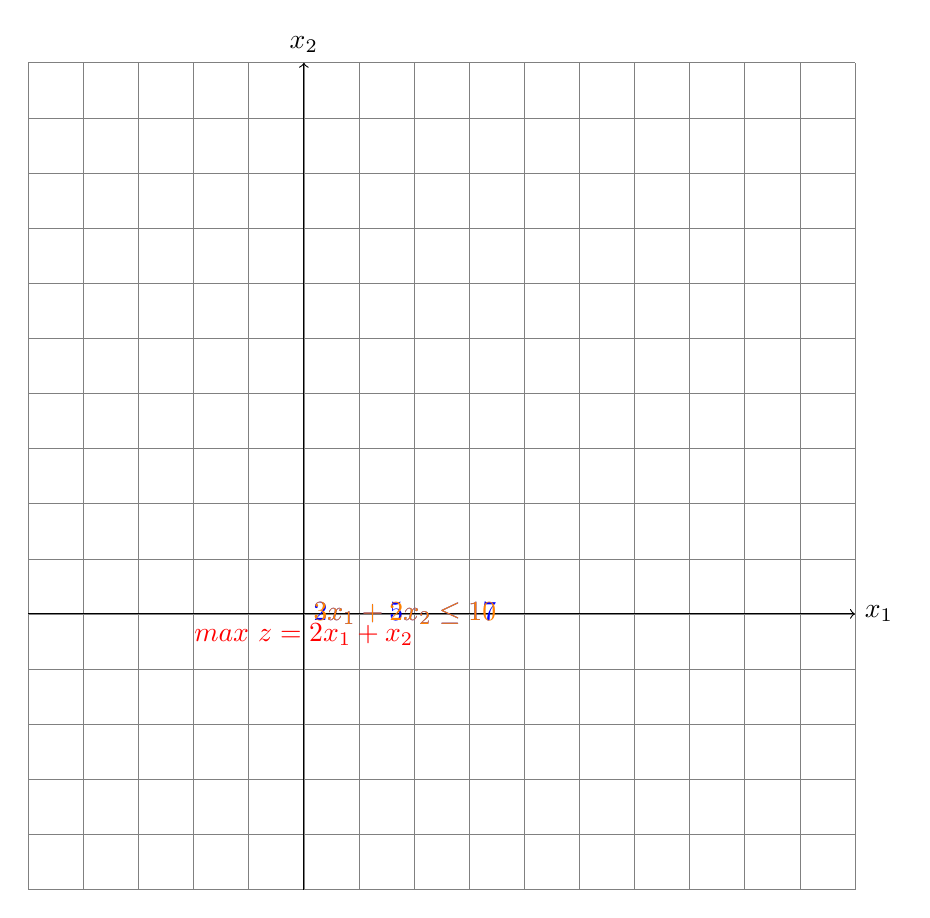
\begin{tikzpicture}[scale = 0.7]

        \filldraw [smooth,draw=gray!20,fill=gray!20] plot[id=f3,domain=0:16.0/11.0]  function {(17.0/5.0) - (2.0/5.0)*x}
            -- (10.0/3.0,0)  -- (0,0) -- cycle;

    \draw[very thin,color=gray] (-5,-5) grid (10, 10);
    \draw[->] plot[id=axeX1] (-5,0) -- (10,0) node[right] {$x_1$};
    \draw[->] plot[id=axeX2] (0,-5) -- (0,10) node[above] {$x_2$};
    
    
    \draw[color=red, domain=-5:2.5, dashed] plot[id=obj] function{-2*x} 
        node[below] {$max\ z = 2x_1 + x_2$};
    \draw[color=blue, domain=-5:10] plot[id=c1] function{(17.0/5.0) - (2.0/5.0)*x} 
        node[right] {$2x_1 + 5x_2 \leq 17$};
    \draw[color=orange, domain=-10.0/3.0:20.0/3.0] plot[id=c2] function{(5.0)-(3.0/2.0)*x)} 
        node[right] {$3x_1+2x_2 \leq 10$};
   	
\end{tikzpicture}


\subsection{Résolution graphique}
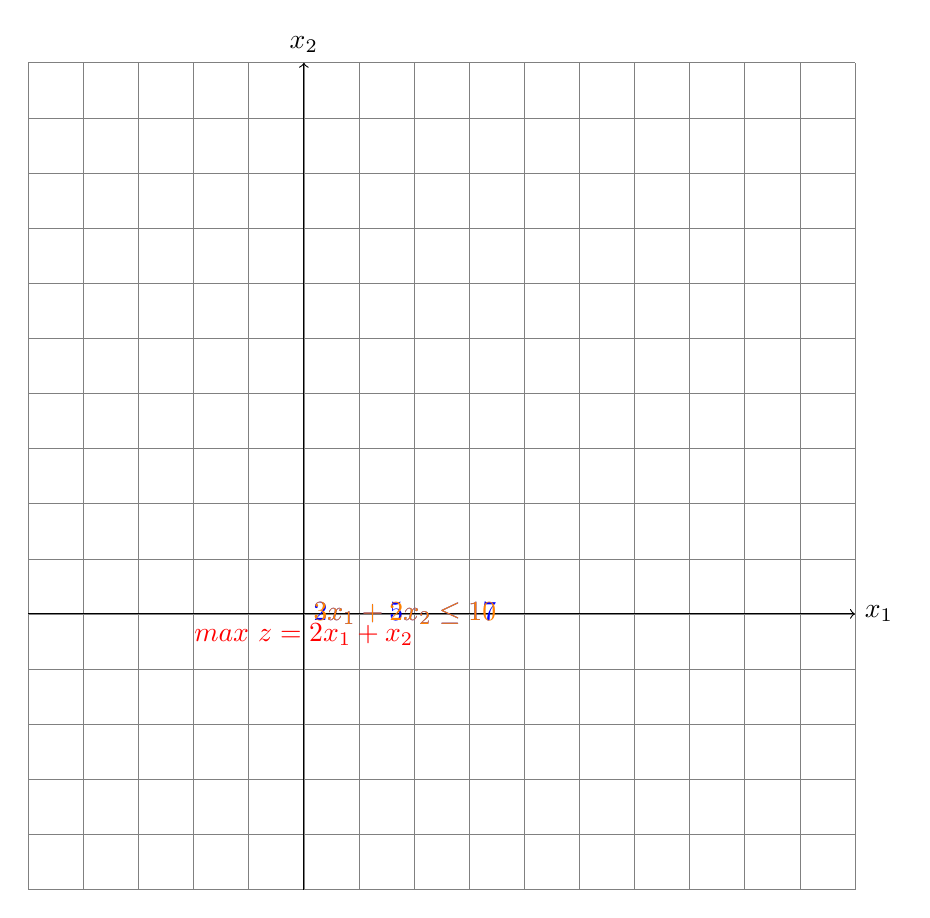
\begin{tikzpicture}[scale = 0.7]

        \filldraw [smooth,draw=gray!20,fill=gray!20] plot[id=f3,domain=0:16.0/11.0]  function {(17.0/5.0) - (2.0/5.0)*x}
            -- (10.0/3.0,0)  -- (0,0) -- cycle;

    \draw[very thin,color=gray] (-5,-5) grid (10, 10);
    \draw[->] plot[id=axeX1] (-5,0) -- (10,0) node[right] {$x_1$};
    \draw[->] plot[id=axeX2] (0,-5) -- (0,10) node[above] {$x_2$};
    
    
    \draw[color=red, domain=-5:2.5, dashed] plot[id=obj] function{-2*x} 
        node[below] {$max\ z = 2x_1 + x_2$};
    \draw[color=red, domain=(-5+1.7):(2.5+1.7), dashed] plot[id=obj] function{17.0/5.0-2*x};
    \draw[color=red, domain=(-5+63.0/22.0):(2.5+63.0/22.0), dashed] plot[id=obj] function{63.0/11.0-2*x};
    \draw[color=red, domain=(-5+10.0/3.0):(2.5+10.0/3.0), dashed] plot[id=obj] function{20.0/3.0-2*x};
        
    \draw[color=blue, domain=-5:10] plot[id=c1] function{(17.0/5.0) - (2.0/5.0)*x} 
        node[right] {$2x_1 + 5x_2 \leq 17$};
    \draw[color=orange, domain=-10.0/3.0:20.0/3.0] plot[id=c2] function{(5.0)-(3.0/2.0)*x)} 
        node[right] {$3x_1+2x_2 \leq 10$};
   	
\end{tikzpicture}

Nous obtenons grâce à la résolution graphique : 
$$ \begin{cases}
x_1 = \frac{16}{11} \\
x_2 = 0 \\
z = \frac{20}{3}
\end{cases} $$


\subsection{Résolution par la méthode du simplexe}
Programme linéaire :
$$
PL_0 \begin{cases}
max\ z(x_1,x_2) = 2x_1 + x_2 \\
 2x_1 + 5x_2 \leq 17 \\
 3x_1 + 2x_2 \leq 10 \\
 x_1, x_2 \geq 0 \\
\end{cases}
$$

Forme standard :
$$
PL_0 \begin{cases}
max\ z(x_1,x_2) = 2x_1 + x_2 \\
 2x_1 + 5x_2 + y_1 = 17 \\
 3x_1 + 2x_2 +y_2 = 10 \\
 x_1, x_2, y_1, y_2 \geq 0 \\
\end{cases}
$$


Tableaux :

$$ \begin{array}{|C{1cm}|C{2cm}|C{1cm} C{1cm} C{1cm} C{1cm}|} \hline
	 &  & 2 & 1 & 0 & 0 \\ \hline
	0 & y_1 = 17 & 2 & 5 & 1 & 0 \\ 
	0 & y_2 = 10 & 3 & 2 & 0 & 1 \\ \hline
	 & z = 0 & -2 & -1 & 0 & 0 \\ \hline
 \end{array} $$
 
 $$ \begin{array}{|C{1cm}|C{2cm}|C{1cm} C{1cm} C{1cm} C{1cm}|} \hline
	 &  & 2 & 1 & 0 & 0 \\ \hline
	0 & y_1 = \frac{31}{3} & 0 & \frac{11}{3} & 1 & -\frac{2}{3} \\ 
	2 & x_1 = \frac{10}{3} &1 &  \frac{2}{3} & 0 & \frac{1}{3} \\ \hline
	 & z = \frac{20}{3} & 0 & \frac{1}{3} & 0 & \frac{2}{3} \\ \hline
 \end{array} $$


\subsection{Recherche d'une solution à valeurs entières}

\subsubsection{Branch and bound}

\subsubsection{Coupes de Gomory}